\documentclass{article}

\usepackage{mathtools}
\usepackage[margin=0.5in]{geometry}
\usepackage{graphicx}
\usepackage{caption}
\usepackage{subcaption}
\usepackage{hyperref}
\usepackage{booktabs}
\usepackage{float}
\usepackage{multirow}

\setlength{\parindent}{0pt}
\graphicspath{ {./experiment/data/} }

\title{Edge Detection Evaluation of HEp-2 Cells in Fluorescent Images}
\author{Ossama Edbali - ID: 1466610}

\begin{document}
	
	\maketitle	
	
	\section{Aim}
	
	This study aims to analyse the results and efficacy of several edge detection algorithms
	on HEp-2 cells.
	
	The edge detection/segmentation algorithms used are: Otsu, Sobel, Roberts, Canny,
	Canny using anisotropic diffusion,
	Laplacian of Gaussian, Difference of Gaussians and dilate-erode method.
	
	The evaluation of each method is carried by ROC curves, sensitivity-specificity variation graphs and correspondence analysis.
	
	\textbf{All the Matlab code and full data can be found here: \url{http://uobcs.github.io/hep2-edge-detection/}.}
	
	\section{Method}

	First of all the experiments where conducted using three main scripts (one for each
	image):
	\verb|x9343AM_task|, \verb|x10905JL_task| and \verb|x43590AM_task|.
	
	Each script loads the relative image and true edge image. Then produces a greyscale image using the \texttt{rgb2gray} Matlab function.
	Finally, it performs all the edge detection algorithms described above (delegating
		to the class \texttt{EdgeDetection.m}).
	A pre-analysis (qualitative) of the input has been carried out using the
	background approximation image as a surface to see where illumination varies (using \verb|show_background| function).
	It can be seen that the various input images are the outcome of different fluorescence patterns on	the HEp-2 cells.
	
	For all edge detectors there is a method inside the \texttt{EdgeDetection} class
	as well as methods for generating the ROC space and specificity and sensitivity
	in function of some parameters (e.g. threshold, sigma, number of iterations).
	
	For Roberts and Sobel a function \verb|detect_edges(img, filterX, filterY)| was developed which convolves \verb|img| with the two filters and uses
	\verb|magnitude| to produce the final result (before thresholding).
	
	In regards to LoG, Gaussian smoothing was performed using \verb|gaussian_smoothing(image, sigma)|. Then convolve the smoothed image with the laplacian
	operator and finally find the zero crossings using \verb|edge(res, 'zerocross')|.
	
	\subsection*{Otsu's method}
	One of the algorithms used in this study is Otsu's algorithm.
	The aim is to find the threshold value where the sum of foreground and background spreads is at its minimum. First of all I calculate the weighted mean and variance
	for both the background and foreground ($\mu_b$, $\sigma_b^2$ and
	$\mu_f$, $\sigma_f^2$). Then I compute the \textbf{within-class variance} (two variances multiplied by their associated weights): $\sigma_W^2 = W_b \sigma_b^2+W_f \sigma_f^2$. I do the same calculation for candidate thresholds and the one that has the lowest within-class variance will be chosen. This algorithm is implemented in Matlab's
	\verb|graythresh|. This will produce a binary image which edges' can be detected
	easily by any of the edge detectors (Sobel in the experiment).
	
	\subsection*{Dilate-erode method}	
	
	The dilate-erode method is a 4-step algorithm that uses a combination of  morphological operators before using Sobel edge detector. The reason why this method
	has been used is that when Sobel (or Roberts) is performed on the greyscale image, there are some lines of high contrast surrounding
	the actual edge (like noise). The gaps between these small lines and the actual edge
	can be filled using a \textbf{dilate morphological operator} (or non-linear neighbourhood
	operator) with a structuring element (from the \verb|strel| function). Then
	\verb|imfill| has been used to fill the holes inside the cell - this step can
	be skipped but it will result in a lower performance.
	The next step is to "reduce" the cell to get it back to its state before
	dilation using
	the \textbf{erosion} operator. Finally the Sobel filter has been used to detect
	edges.
	There are various ways to create the  morphological operators. Here is the one
	used in this study (erode example using a 5x5 mask): \verb|erode = @(x) min(x(:)); out = nlfilter(in,[5 5],erode)|.
	
	\subsection*{Canny with anisotropic diffusion (CAD)}	
	
	From the study it has been noted that Canny performed with sensitivity lower than
	0.4 in all input images. To enhance the images but still preserving true edges,
	\textbf{anisotropic diffusion} has been used.
	Anisotropic diffusion is a non-linear diffusion filtering for avoiding the
	blurring problems of Gaussian smoothing (and others). It is an iterative
	process to perform edge-preserving smoothing on the cells.
	The algorithm is described mathematically as follows:
	
	\begin{center}
	$\frac{\partial}{\partial t}I(x, t) = \nabla \bullet (c(x, t) \nabla I(x, t))$
	\end{center}		
	
	Here $t$ is the iteration step, $c(x, t)$ is a decreasing diffusion function
	of the image gradient magnitude.
	
	The \verb|anisodiff2D(im, num_iter, delta_t, kappa, option)| function in the codebase
	has been implemented to accomplish anisotropic diffusion. Here \verb|im| is the
	input image, \verb|num_iter| is the number of iterations, \verb|delta_t| is
	the integration constant, \verb|kappa| is the diffusion constant and
	\verb|option| defines which diffusion function to use.
	\newline
	
	I adopted three evaluation methods in order to assess the accuracy/efficacy of each edge
	detector technique:
	
	\subsection*{ROC curve}
	
	The ROC curve has been used to detect which parameter to choose according
	to a \textbf{diagnosis line} (in the experiment
	(0, 1) to (1, 0) has been used). The implementation can be found under
	the \verb|compute_roc(ID, IT)| function, where ID is the image
	with detected edges and \verb|IT| is the image with true edges.
	Basically it takes the two binary images and performs logical operations
	for all possible cases (e.g. true positive, false positive etc\ldots) and
	calculates the sum of "on" pixels in the resulting images. Then it combines
	the results to find sensitivity and specificity:
	
	\begin{center}
	\verb|sensitivity = TP / (TP + FN)| and \verb|specificity = TN / (TN + FP);|
	\end{center}
	
	\subsection*{Sensitivity/Specificity variation}	
	
	This evaluation method simply uses the sensitivity and specificity parameters in function
	of a variable (threshold, sigma, kappa or number of iterations). From this we
	can see how different algorithms respond to the variation of some parameters.
	This is implemented by the \verb|roc_params_comparison| static method in the
	\verb|EdgeDetection| class.
	
	\subsection*{Correspondence analysis (intra-method analysis)}	
	
	From $N$ edge detection results (using the same edge detector) test for
	correspondence as follows: a pixel location identified as an edge by
	all $N$ detector configurations (i.e. changing parameter)
	will have the highest correspondence ($N$), and a
	location identified as an edge by only one detector setup will have the lowest.
	
	This is computed by the \verb|correspondence_analysis| function in the codebase which
	adds all the input image matrices and, using Matlab's \verb|bar|, plots a bar diagram
	with frequencies for each correspondence level (using \verb|histc|).
	
	\section{Results}
	
	A very interesting result is the comparison between Canny and Canny with anisotropic diffusion (using 9343 AM as a reference).

\begin{figure}[htp]

\centering
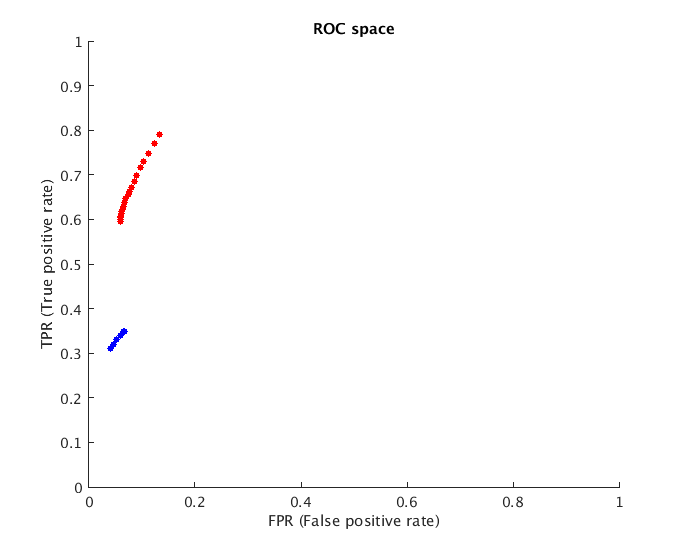
\includegraphics[width=.3\textwidth]{x9343AM/comparison.png}\hfill
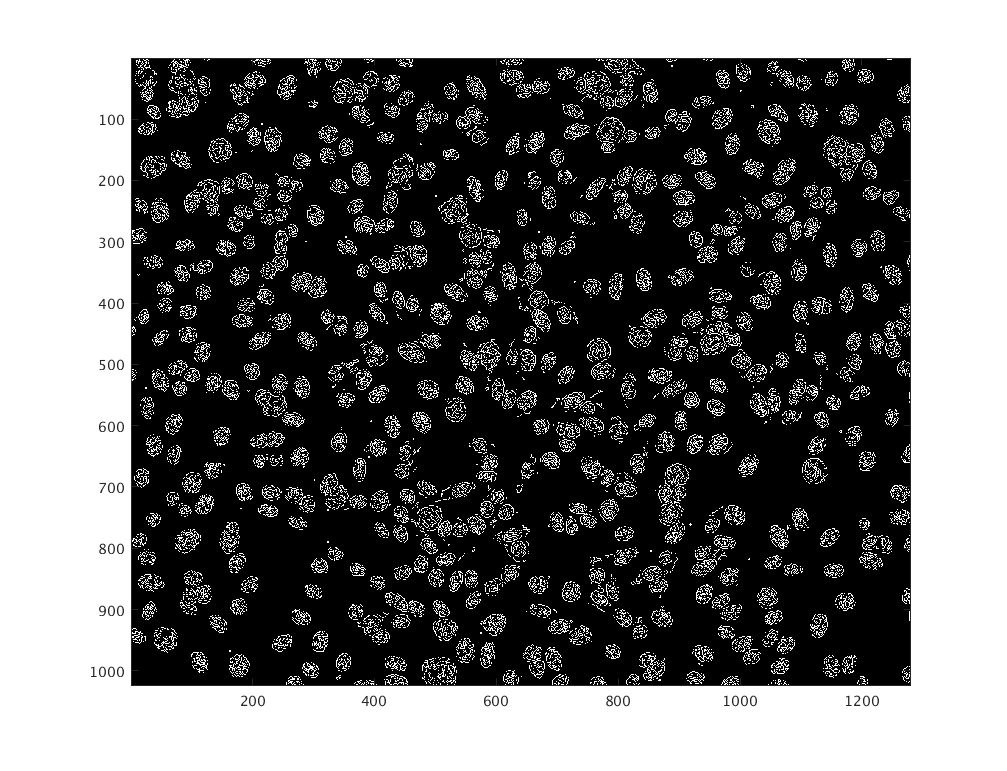
\includegraphics[width=.3\textwidth]{x9343AM/canny/result.png}\hfill
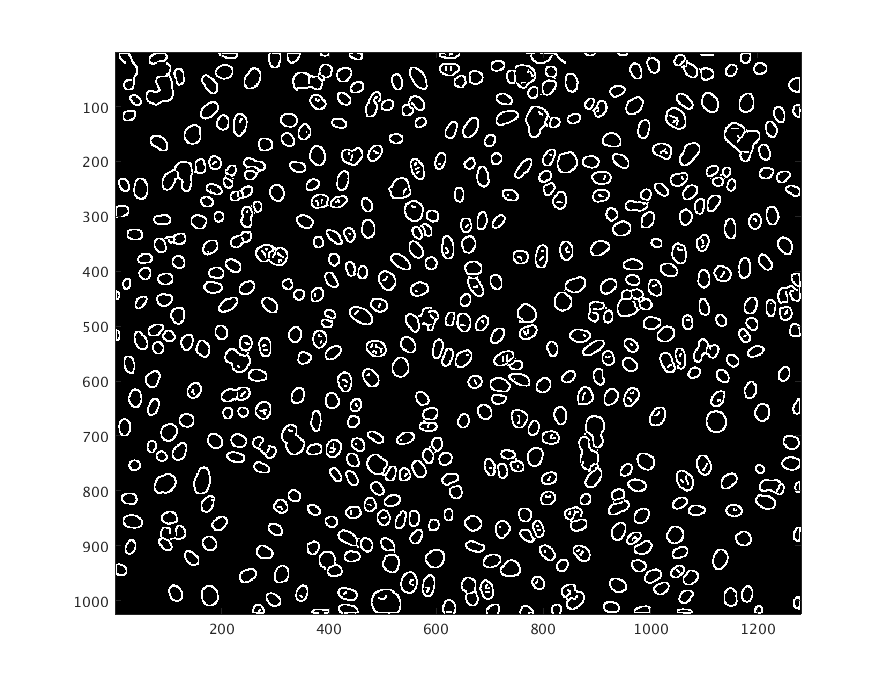
\includegraphics[width=.3\textwidth]{x9343AM/cad/result_15_iterations.png}

\caption{(1) ROC space comparison, (2) Canny, (3) Canny with anisotropic diffusion }
\label{fig:figure3}

\end{figure}
	
	It can be noted that Canny does not perform very well (sensitivity under 0.4).
	However if we apply anisotropic diffusion,
	sensitivity drastically increases (over 0.8). This happens because the input image
	is very dark at the borders and Canny looses information in the smoothing
	step as well as in the non-maximum suppression step. Supporting this statement
	are the results of applying Canny to 43590 AM (which is very dark compared to
	the other two images and therefore a high smoothing).
	
	A summary of the whole data using the optimal parameters (\textbf{for the FULL evaluation graphs, tables and image results please visit this site: \url{http://uobcs.github.io/hep2-edge-detection/}}):
	
\begin{table}[H]
\centering
\caption{Overall results (1: 9343 AM, 2: 10905JL, 3: 43590AM)}
\label{my-label}
\begin{tabular}{|c|c|l|l|}
\hline
\multicolumn{1}{|l|}{Edge detector} & \multicolumn{1}{l|}{Image} & Sensitivity & Specificity \\ \hline
\multirow{3}{*}{Otsu}               & 1                          & 0.9225      & 0.9974      \\ \cline{2-4} 
                                    & 2                          & 0.9279      & 0.9957      \\ \cline{2-4} 
                                    & 3                          & 0.8813      & 0.9958      \\ \hline
\multirow{3}{*}{Sobel}              & 1                          & 0.8498      & 0.8638      \\ \cline{2-4} 
                                    & 2                          & 0.8953      & 0.8852      \\ \cline{2-4} 
                                    & 3                          & 0.8195      & 0.8237      \\ \hline
\multirow{3}{*}{Roberts}            & 1                          & 0.8477      & 0.8400      \\ \cline{2-4} 
                                    & 2                          & 0.8646      & 0.8779      \\ \cline{2-4} 
                                    & 3                          & 0.7540      & 0.8215      \\ \hline
\multirow{3}{*}{Canny}              & 1                          & 0.3404      & 0.9408      \\ \cline{2-4} 
                                    & 2                          & 0.3057      & 0.9863      \\ \cline{2-4} 
                                    & 3                          & 0.2396      & 0.9808      \\ \hline
\multirow{3}{*}{CAD}                & 1                          & 0.7910      & 0.86651     \\ \cline{2-4} 
                                    & 2                          & 0.8139      & 0.9204      \\ \cline{2-4} 
                                    & 3                          & 0.6734      & 0.8921      \\ \hline
\multirow{3}{*}{Dilate-Erode}       & 1                          & 0.8299      & 0.8058      \\ \cline{2-4} 
                                    & 2                          & 0.8003      & 0.8119      \\ \cline{2-4} 
                                    & 3                          & 0.7446      & 0.7863      \\ \hline
\multirow{3}{*}{LoG}                & 1                          & 0.2250      & 0.9419      \\ \cline{2-4} 
                                    & 2                          & 0.2135      & 0.9324      \\ \cline{2-4} 
                                    & 3                          & 0.1996      & 0.9207      \\ \hline
\multirow{3}{*}{DoG}                & 1                          & 0.2137      & 0.9857      \\ \cline{2-4} 
                                    & 2                          & 0.2446      & 0.9941      \\ \cline{2-4} 
                                    & 3                          & 0.17301     & 0.99094     \\ \hline
\end{tabular}
\end{table}
	
\begin{table}[H]
\centering
\caption{Otsu evaluation}
\label{otsu}
\begin{tabular}{@{}llll@{}}
\toprule
Image    & Sensitivity & Specificity & Threshold \\ \midrule
9343 AM  & 0.9225      & 0.9974      & 0.0902    \\
10905 JL & 0.9279      & 0.9957      & 0.1333    \\
43590 AM & 0.8813      & 0.9958      & 0.0510    \\ \bottomrule
\end{tabular}
\end{table}

Overall Otsu has proven to be the best choice in all the images. Although
computationally expensive, Otsu's method takes into account foreground and
background and gives satisfactory results only when the numbers of pixels in each class are close to each other (which is the case here).

Sobel and Roberts have performed almost equally in all images however Sobel has
higher specificity because it is less sensitive to isolated high intensity point variations. Thus it gives correct results when the edge do not exist in a given point.

In regards to the dilate-erode method
we can notice that the sensitivity decreases very fast compared to Sobel (or Roberts). This is because during the erode process some edges might be removed and this propagates to the Sobel edge detection and thresholding.


	
	\section{Conclusion}
	
	In this study various alternatives to the traditional edge detectors have been
	tried because of their specific application to cell edge detection. For example
	Canny is very sensitive to the fluorescence around the cells. LoG and DoG have
	low sensitivity (for optimal parameters) because they highlight regions
	of rapid intensity changes but the input images have gradual
	change from the cell to the background (fluorescence effect). Some extensions to
	the edge detectors (such as dilate-erode, adjust and anisotropic diffusion)
	have proven to increase the efficacy of the edge detection.
	
\end{document}